\documentclass[output=paper]{langscibook} 
\author{Dolors Font-Rotchés\lastand Francisco José Cantero Serena\affiliation{Universitat de Barcelona}}
\title{Melodic Analysis of Speech: Phonetics of Intonation}
% \chapterDOI{} %will be filled in at production
%\affiliation{University of Barcelona}

\abstract{The acoustic-perception based on the Melodic Analysis of Speech method (MAS) is a formal, objective and complete method that encompasses the most relevant aspects to be considered when analysing intonation. It provides researchers who wish to study intonation with criteria for establishing a corpus, the identification of melodic units, the extraction and relevance of acoustic data, its standardisation and the representation and interpretation of graphs, as well as the execution of perception tests and validation of the results obtained. It also offers a way of interpreting the melodic data based on three levels of intonation: one which provides an explanation of the speech, the prelinguistic level, the linguistic level and the paralinguistic level, which gives it significance with regard to the speaker's intentions or the communicative context. In addition, a phonological description based on the Autosegmental-Metrical model (AM) and its labelling convention known as Tones and Break Indices (ToBI), which is complementary and totally compatible with the phonetic description of MAS, can be added.The method, proposed in \citet{CanteroSerena.1999,CanteroSerena.op.2002}, tested and expanded in \citet{FontRotches.2007} and established as a protocol in \cite{Cantero2009}, is not a closed model but one that is constantly advancing, being reformulated and added to as new requirements arise resulting from its use by researchers in the description of different languages, interlanguages and dialects. It is these developments, which have occurred over more than a decade and particularly in the last two years, together with the basic pillars of the method, which are presented in this article.}
\maketitle

\begin{document} 
\label{chap:font}
% \textbf{Keywords:} Melodic Analysis of Speech method, Intonation, Acoustic analysis, Perception tests, semi-automatic analysis.

\section{Introduction}

This paper presents the most relevant characteristics of the Melodic Analysis of Speech (MAS) method, together with the developments that have taken place to date.\footnote{This paper is part of the research project financed by the Ministry of Economy and Competitiveness \textit{Analysis of Speech and Teaching Models}, ref. FFI2013-41915-P.} It was proposed by \citeauthor{CanteroSerena.1999} in \citeyear{CanteroSerena.1999}, published in \citeyear{CanteroSerena.op.2002} and since then, has been used by various researchers, initially to describe languages and interlanguages and later dialect variants and aspects of paralinguistic intonation (in relation to the speaker's intentions and the communicative context). Currently, there are open lines of research on description and analysis relating to different aspects of intonation in different languages. 

Traditionally, intonation has been one of the aspects of speech characterisation that has been greatly ignored by linguists. The first people to show an interest in describing intonation were authors from the \textit{British school}. Authors such as \citet{Jones.1909,Palmer.1922}, and \citet{Armstrong.1926} aimed to write manuals designed for the correct teaching of English. In their work, they provided melodic curves, their context and meaning, so that learners could imitate them. In later decades, other linguists followed this tradition, including \citet{OConnor.1961,Crystal.1969,Cruttenden.1986} and the American, \citet{Bolinger.1986,Bolinger1989}. Close to this tradition, although with original contributions that have greatly influenced intonation studies for the Spanish language, \citeauthor{NavarroTomas.1944} published his \textit{Manual for Spanish Intonation} in 1944, designed as a practical language manual and a theoretical treatise on Spanish intonation.

Also based on the phonetic characterisation of intonation, authors of the Dutch school, \citet{Hart.1990} and their \textit{IPO model} (Institute for Perception Research) are of note, as they provide a stylisation of the intonation curves through the selection of relevant pitch movements in the melodic curve, eliminating other pitch variations.

At the same time as these schools, from a structural perspective of the phenomenon and a phonological viewpoint, linguists of the \textit{American tradition} e\-merged with their level analysis proposal; authors such as \citet{Pike.1945} and \citet{Trager.1951}, among others, described the curve based on four pitch levels, four stress levels (primary, secondary,...) and junctures (marking the beginning and ending of the phrase). 

Along this baseline of phonology, and from the theoretical approach of generative phonology, stems the \textit{Autosegmental and Metrical model} \citep{Pierrehumbert1980,Pierrehumbert.1987}, which, based on the metrical structure of the phrase, suggests the representation of its pitch variations using two levels: H (high) and L (low). For this model, during the 1990s, the ToBI (Tone and Break Indices) transcription system was developed for English (\citealt{Silverman1992,BeckmanHirschberg1994}), as well as systems for other languages, including Italian (ToBIt, \citealt{Avesani1995}), German (GToBI, \citealt{Grice.1996}) and Spanish (Sp-ToBi, \citealt{Beckman.2002}), among others, and a transcription variant for Dutch (ToDI, \citealt{Gussenhoven.1999ToDI}).

Later, and influenced by the Autosegmental-Metrical model, the Aix-en-Pro\-vence model emerged, also generative, which suggested obtaining phonological forms of the prosodic system of different languages. To do so, they follow an automatic styling process using the MOMEL (MOdelling MELody) algorythm and the INTSINT notation model \citep{Hirst2000}. 

In this context, the \textit{Melodic Analysis of Speech} (MAS) model aims to provide a robust approach for the acoustic analysis of intonation, regardless of its phonological interpretation. It is a formal and objective method that provides the researcher with a way of analysing intonation, described in detail in the protocol established in 2009 by Cantero and Font-Rotchés\footnote{There is an English version in \citet{Cantero2009}.} and also with a way of interpreting the data from different levels of intonation (prelinguistic, linguistic and paralinguistic), developed in \citet{CanteroSerena.op.2002}.

The protocol is divided into three sections: the identification of melodic units in a corpus of spontaneous speech, the development of an acoustic phase, including the determination of relevant frequency values and standardisation and lastly, a perception phase, during which the analyses and interpretation of data is validated. It remains the same for the procedure described below, although with some new contributions resulting from research, such as matters regarding labelling or the relevance of a number of values in the analysis that have proven to be important for some levels of intonation. Other significant developments include the creation of the semi-automated script by \citet{MateoRuiz.2010Scripts}, which has also evolved over the years, adapting to the requirements of the group's research. 

With regard to levels of intonation, in the prelinguistic level (melodic features that structure the discourse and delimit it in comprehensible units), motivated by the development of several studies on dialect variants and interlanguages, the new term, \textit{melodic profile}, has been coined and defined as a series of melodic features that characterise an ``accent'' (such as dialect or foreign accent). On a paralinguistic level, three types of intonation have been defined: emotional, focus and (im)politeness. And finally, given that some melodic features simultaneously inform us of different characteristics (dialect or interlanguage, linguistic or pertaining to the speaker's intentions or the communicative context), the term \textit{melodic syncretism} has been coined, which will be developed further in future research.

Therefore, the following sections explain the steps to be followed for applying the method, which include all of the developments made to date and the interpretation of melodic data, as well as a final discussion chapter where current research being made is described and some possible additions to the method in the near future are set forth.

\section{Identification of melodic units}
\label{sec:fon:2}
\subsection{Phonic hierarchy}
Sounds of speech do not occur indiscriminately but are organised in phonic blocks around accents, which are the true nuclei of discourse and have a hierarchical relationship, called \textit{phonic hierarchy} \citep{CanteroSerena.op.2002}, shown schematically in \figref{fig:font:1}. 

{According to this hierarchical relationship, consonant sounds are organised around vowel sounds creating syllables and these join together to form words for which the stress is the most relevant component (e.g. the syllable \textit{par}- in \textbf{\textit{par}}\textit{que}). This  stress is not only combined with the  unstressed syllables of the word but also by adjacent unstressed words, such as prepositions, articles, conjunctions, unstressed pronouns, etc. to create  \textit{phonic words} or \textit{rhythmic groups} (e.g. \textit{por el} \textbf{\textit{par}}\textit{que}, where \textit{par}- is the nucleus).}

{Phonic words or rhythmic groups as a whole also form blocks around an accent, which stands out and is higher in the hierarchy. These create the \textit{phonic group} or ``the major phonic unit that segments the discourse and the only one that has its own identity and is not conditional upon other units'' \citep[83]{CanteroSerena.op.2002}. The accent or nucleus of the phonic group, which is the most relevant, is normally found on the last phonic word (e.g. the syllable \textit{par}- of the phonic group \textit{Ayer paseábamos por el} \textbf{\textit{par}}\textit{que}).} 

\newcommand{\fb}[2][1.7cm]{\framebox{\parbox{#1}{#2}}}
\newcommand{\ub}[2]{\underbrace{#1}_{\text{#2}}}
\begin{figure} 

\includegraphics[width=0.99\textwidth]{figures/FON-img1.PNG}

%$
%\ub{
%  \ub{
%    \ub{
%      \ub{
%	\fb{voiceless\\consonant}~\fb{voiced\\consonant}~\fb[1cm]{glide\\~}}{~}
%      \fb[1cm]{atonic\\vowel}}{Syllable}
%    \fb[1cm]{tonic\\vowel}}{Phonic word}
%  \fb[2.5cm]{tonic vowel\\with inflection}}{Phonic group}
%$
 

\caption{\label{fig:font:1} Diagram of phonic hierarchy.}
\end{figure}

{The way of organising speech or phonic hierarchy comprises the personality of each language beyond the mere pronunciation of sounds and has two functions. On the one hand, it integrates the sounds organised hierarchically and forming phonic blocks (syllables, rhythmic groups and phonic groups) by the speaker and on the other it delimits these phonic blocks and allows recognition of the words in each block facilitating comprehension of the discourse by the listener.} 

\subsection{Melodic units}
The phonic group, which we have defined as the major phonic unit of discourse, where sounds of the language are organised hierarchically and within which the rhythmic structure of the discourse is established, contains a coherent lexical-grammatical structure together with a melody. This melody, which represents a significant melodic unit in the intonation of speech, is called the \textit{intonation contour}. 

The smallest melodic unit of the intonation contour is the \textit{tonal segment}, in other words, each one of the more or less stable and perceptibly clear phases, which tend to coincide with a \textit{mora} (equivalent to the duration of a short vowel). In this regard, a vowel tends to last a mora and therefore contains a tonal segment, whilst a long vowel, such as the tonic vowel where the nucleus of the phonic group occurs tends to last for two moras and as a result contains two tonal segments with different tonal values. This succession of two adjacent and different tonal segments is what we call \textit{tonal inflection}.

The different values of the tonal segments that comprise the melody of the intonation contour follow the hierarchy of the phonic group. Therefore, the only tonally relevant segments are the vowels (these comprise an identifiable tonal segment in the melody of the contour) and, particularly, the tonics (nuclei of rhythmic groups), which stand out among the atonics because they present a tonal contrast. Unlike vowels, voiceless consonants are not sounds but noises because they lack phonation, whilst voiced consonants or glides, despite being considered as sounds, tend to be marginal because they always occur associated with a vowel. Among the different nuclei of rhythmic groups that form a phonic group there is one that stands out for containing the most relevant accent or \textit{nucleus}, melodically characterised for including a tonal inflection with two tonal segments and usually found in the last rhythmic group. Similarly, the first tonic vowel of the contour or \textit{first peak}, is particularly relevant.

Following this hierarchy of the phonic group, which contains the intonation contour, we can see, in \figref{fig:font:2}, that its structure is divided into three parts: the \textit{anacrusis}, the \textit{body} or  \textit{declination} and the \textit{final inflection (FI)}, limited by two accents, the \textit{first peak} \textit{(1st peak)} and the \textit{nucleus}. By \textit{anacrusis} we understand the unstressed syllables prior to the first stressed vowel in the contour, called the \textit{first peak,} and by \textit{body,} the syllables from the first peak to the last stressed vowel in the contour, called the \textit{nucleus}, the point from which the \textit{final inflection} begins. The description of these elements (especially the description of the \textit{final inflection}) allows us to define the contour melody.

\begin{figure}
\includegraphics[width=.7\textwidth]{figures/FON-img2.PNG}
\caption{Diagram of the three parts of the contour.}
\label{fig:font:2}
\end{figure}

To obtain the melodic units or intonation contours of a spontaneous speech corpus, initially choosing the utterances that coincide with a turn to speak in the dialogue (normally short and easy to identify) is advisable, until the researcher has acquired enough confidence in identifying phonic groups and in defining speech melodies. However, it is not always possible to select a turn from the dialogue. For this reason, to identify phonic groups we use the nucleus of the phonic group as a formal criterion for segmenting speech. This nucleus is the accent that has a tonal inflection and is the most significant part of the contour, tending to occur on the last phonic word. 

\subsection{Establishing the corpus}
\label{sec:font:2.3}
To establish a corpus for the purpose of describing a language or a dialect variant, models of spontaneous speech must be obtained that provide an intonation reality, in other words, fragments of speech, uttered by speakers who produce them in a real context. For this reason, the corpus must be obtained from outside of the laboratory and without any prepared or induced written or spoken support from the researcher (see \citeauthor{GarridoAlminana.2018}, \citeauthor{TeixeiraKalkhoff.2018} and \citeauthor{Peskova.2018}, this volume, for more information about large corpora and spontaneous speech in the study of prosody). 

It must also include a significant number of speakers, who vary in regard to age, gender and social-cultural background, who have no speech impediments and who are native speakers of the language. 

In certain types of TV programmes such as talk shows, street interviews, debates, discussions and game shows, among others, we have found a resource that meets these basic requirements: multiple native and anonymous speakers of a language who spontaneously express themselves in a context of dialogue. It is worth mentioning that when selecting them we avoid professional speakers and all TV show hosts who follow a script or who are reading, so as to ensure that the utterances of the corpus are produced by speakers in a spontaneous context. 

Another point to be considered regarding the selection of the utterances is that, in addition to being produced naturally in a real conversation, there must be no overlapping of voices or background noise or music that impede analysis. First interventions by speakers are also disregarded as these could be prepared, selecting those expressed in an uninhibited way and with no form of prior preparation. 

Each utterance chosen must be coded, which includes noting down the transcription, its location on the recording, identifying data of the television programme (as well as the time and day it was broadcast) and, where appropriate, the type of recording, a description of the conversational context in which the utterance was produced and information about the speaker. 

Once the utterances have been selected and coded, the audio is extracted from the video using suitable software. Afterwards it is segmented in Praat and given a code. It is worth noting that a maximum of ten utterances per speaker is established so that the corpus is as varied as possible.

Meeting these requirements is the corpus of Peninsular Spanish by \citet{Alfonso.1999}, which does not distinguish the origin of the speakers and includes a total of 90 utterances produced by 37 speakers. Years later, corpora were created by \citet{BallesterosPanizo.2011} and \citet{MateoRuiz.2014}, each including samples from five different regions: Asturias, Navarre, the Basque Country, Castile-Leon and Madrid in the case of Ballesteros and Andalusia, the Canary Islands, Castile-La Mancha, Extremadura and Murcia in the case of Mateo. In total the two corpuses include 373 hours of recordings, 2941 utterances and 814 speakers \citep{CanteroSerena.2016}.

These corpuses are the ones used to characterise the linguistic intonation of spontaneous speech in \citet{CanteroSerena.op.2002,CanteroSerenaETAL.2005,CanteroSerena.2007} and \citet{FontRotches.2013b}, as well as the dialect intonation in \citet{BallesterosPanizo.2011} and in \citet{MateoRuiz.2014}. In addition to being useful for describing aspects of intonation, they have also served as a basis for acoustic analyses focussing on the pronunciation of Spanish, regarding vocalism \citep{Alfonso.2010} and lateral \citep{Andres.2014}, vibrant \citep{OrtizdePinedoSanchez.2012} and approximant \citep{SolaPrado.2011,SolaPrado.2014} sounds.

Also of note is the Catalan corpus by \citet{FontRotches.2006}, which includes 46 hours of recording, 580 utterances and 160 speakers. This corpus, apart from being useful for describing the linguistic intonation of Catalan \citep{FontRotches.2007} and emphatic intonation \citep{FontRotches.2011}, has also been used to describe the intonation of (im)politeness \citep{DevisHerraiz.CanteroSerena.2014} and the vocalism of Catalan \citep{RiusEscude.2015}.

Following this same protocol for creation, there is also a corpus of spontaneous speech of German \citep{TorregrosaAzor.2011}, Brazilian Portuguese \citep{Araujo.2014,Mendes.2013} and Chinese \citep{Kao.2011}. 

Other types of corpus also exist that have different objectives, such as the description of an interlanguage, which implies creating a corpus following different criteria to those indicated for spontaneous speech.

In studies carried out by our group on interlanguage, understanding interlanguage to be the different phases of development in the acquisition of a foreign language or L2 by a speaker (a term coined by \citealt{Selinker.1972}), corpora have been created using other strategies for their characteristics. In research on Spanish spoken by Taiwanese people \citep{Liu2005}, Hungarians \citep{BaditznePalvoelgyi2012}, Brazilian Portuguese speakers \citep{FonsecadeOliveira.2013} and Swedish \citep{Martorell.2010}, conversations between the interlanguage speakers have been recorded using microphones outside a laboratory environment — sometimes this involved a Spanish learning classroom activity, sometimes in different situations — and focusing the interest on the content: personal experiences, opinions of their relationship with the Spanish language and culture or on hot topics in current affairs, among others, with the aim of obtaining conversations that are as spontaneous as possible. 

And lastly, with regard to describing models of speech by television news readers, advertising actors and current affairs programme presenters, who produce a very formal and media-oriented model of speech from a written text, a corpus has been created taken from recordings of television broadcasts of each one of these genres (see \citealt{FontRotchesPaloma.2013} and \citealt{Torrent.2012,Torrent.2015} for Catalan and \citealt{FontRotchesMachucaAyuso.2010,FontRotches.2011} for Spanish). 

\section{Acoustic phase}
\subsection{Determination of relevant frequency values} 

Once the utterances have been separated, we establish the F\textsubscript{0} value of each vowel, of each tonal segment. This involves differentiating the relevant frequency values (the tonal segments) from the irrelevant values (the F\textsubscript{0} of the sonorous consonants and of the glides). This is done using Praat analysis and synthesis software \citep{Boersma.praat}, which is a reliable acoustic analysis instrument.

We identify the vowels (guided by a sonogram) and establish their value (the average of the F\textsubscript{0} values of the vowel. \figref{fig:font:3} shows an example of the extraction of frequency values of the utterance \textit{Tiene usted hijos?} ‘Do you have any children?’ obtained by using the \textit{Praat} application. The dark areas of the spectrogram correspond to each one of the vowel segments (or diphthongs) and for each one of them the F\textsubscript{0} value in Hz is obtained from the average value of the vowel’s F\textsubscript{0} (e.g. \textit{-ie-}, \textit{-e-, -u-, -e-}, -\textit{i}- and \textit{-o-} in \figref{fig:font:3}).

\begin{figure}
\includegraphics[width=\textwidth]{figures/FON-img3.PNG}
\caption{\label{fig:font:3} Extraction of frequency values of the utterance} ¿Tiene usted hijos? ‘Do you have children?'
\end{figure}

When a stressed vowel contains a tonal inflection with a tonal distance of at least 10\%\footnote{This tonal distance has been verified in different perception tests carried out by the Applied Phonetics Lab of the University of Barcelona and applied in MAS research since 2011 and it is the result of calculating a percentage of a distance between the initial and final values of a vowel, e.g .\textit{hi}-, from 293 Hz to 376 Hz, in \figref{fig:font:3} and \tabref{tab:font:4} or \textit{Stadt}, from 169Hz to 195 Hz, in \tabref{tab:font:1} \textit{Cal la traducció d’Stadt}.} (100\% is equivalent to an octave of the musical scale), a value of two tonal segments must be established (see syllable -\textit{hi}- in \figref{fig:font:3} and values in \tabref{tab:font:4}, ), constituting the inflection or three segments if it is a circumflex inflection (see syllable -\textit{xò} in \tabref{tab:font:2}) which can be found in any part of the contour. These values are calculated from the initial and final stable values or from the extreme values of the inflection (if there is no tonal stability). Furthermore, when the inflection ends with a vowel followed by a voiced consonant (specially a nasal, a lateral or a vibrant) with a tonal distance of at least 10\% (see an example in \tabref{tab:font:5}), this consonant usually represents the last tonal segment of the inflection (see perception tests in \citealt{FontRotches.2007}). 

Initially, to describe linguistic intonation we only used very marked tonal inflection data, with more than 20\% of movement. However, for research on dialects and interlanguages the need to use data on these inflections with a tonal distance of 10\% for intonation relevance became evident. It is in these small features where some of the characteristics lie that allow us to describe and distinguish one dialect from another (see \citealt{BallesterosPanizo.2011,MateoRuiz.2014}) or to describe the transfer features of the interlanguage from the language of origin, as is the case of Brazilian Portuguese \citep{FonsecadeOliveira.2013} and Italians \citep{DevisHerraiz.2011didactica} speaking Spanish.

With regard to the extraction of tonal values for the final inflection, in other words, the inflection that occurs  in the last tonic syllable of the contour, we can see that there are small variations according to whether the word is oxitonic,  paroxitonic or proparoxytonic. If the word is oxytonic, it may be that the accented syllable has a tonal inflection with two values — we distinguish the second with one asterisk (*), as occurs on the syllable \textit{Stadt} in German, found in the utterance \textit{Schon viel Spass gehabt in der Stadt}? ‘Did you have a good time in the city?’ (see \tabref{tab:font:1}). Where this syllable only has one value, the final inflection would begin on the preceding syllable.

\begin{table}
\begin{tabularx}{\textwidth}{Xcccccccc}
\lsptoprule
Utterance & {Schon} & {viel} & {Spass} & {(ge)habt} & {in} & {der} & {\textbf{Stadt}} & {\textbf{Stadt}}\textbf{*}\\
Hertz & 149 & 172 & 190 & 176 & 164 & 146 & 169 & 195\\
\lspbottomrule
\end{tabularx}
\caption{\label{tab:font:1}Example of German whose last stressed vowel has two values.}
\end{table}

See \tabref{tab:font:2}, with the Catalan example of \textit{Bé, crisi és això!} 'Well, crisis is that!' where the last stressed vowel, -\textit{ò}, has a tonal inflection with three values distinguished by asterisks (*) — one if it is the second value and two if it is the third.

\begin{table}
\begin{tabularx}{\textwidth}{Xcccccccc}
\lsptoprule
Utterance & {Bé} & {cri} & {si} & {és} & {ai} & {\textbf{xò}} & {\textbf{xò*}} & {\textbf{xò**}}\\
Hertz & 328 & 347 & 400 & 365 & 340 & \textbf{316} & \textbf{426} & \textbf{292}\\
\lspbottomrule
\end{tabularx}
\caption{\label{tab:font:2}Example of Catalan whose last stressed vowel has three values.}
\end{table}

On other occasions, the final inflection begins with a stressed vowel and ends with an unstressed vowel, for example, in final inflections that coincide with a word with the stress on the penultimate or antepenultimate syllable. See \tabref{tab:font:3}, the German example of \textit{Kommt das aus Amerika?} ‘Is this from America?’, where the stress is on the antepenultimate syllable.

\begin{table}
\begin{tabularx}{\textwidth}{X*{7}{c}}
\lsptoprule
Utterance & Kommt & das & aus & A & \textbf{me} & \textbf{ri} & \textbf{ka}\\
Hertz & 259 & 323 & 269 & 234 & \textbf{217} & \textbf{296} & \textbf{443}\\
\lspbottomrule
\end{tabularx}
\caption{\label{tab:font:3}Example of German in which the final inflection takes place in a \textit{proparoxytone word}.}
\end{table}

It is also possible for the accent to be found on the penultimate syllable and that this syllable or the following atonic syllable could have two values, therefore giving us a circumflex final tonal inflection with three values, such as the Spanish example in \tabref{tab:font:4} of \textit{¿Tiene usted hijos?} ‘Do you have sons and daughters?' in which the final inflection has three values: the first and the second in the stressed vowel, \textit{hi-} (293 Hz and 376 Hz), and the third in the next unstressed syllable: -\textit{jos} (305Hz).

\begin{table}
\begin{tabularx}{\textwidth}{X*{7}{c}}
\lsptoprule
Utterance & {Tie} & {ne} & {us} & {ted} & {\textbf{hi}} & {\textbf{hi*}} & {\textbf{jos}}\\
Hertz & 256 & 270 & 289 & 295 & \textbf{293} & \textbf{376} & \textbf{305}\\
\lspbottomrule
\end{tabularx}
\caption{\label{tab:font:4}Example of Spanish of a circumflex final tonal inflection.}
\end{table}

There is another Spanish example in \tabref{tab:font:5} \textit{¿Tú tienes internet, Carmen?} 'Do you have internet, Carmen?' in which the final inflection also has three values: the first in the stressed vowel, \textit{Car-}, and the second and the third in the next unstressed syllables: -\textit{men} (123 Hz) from the vowel and -\textit{men}* (159 Hz) from the voiced consonant \textit{-n}.

\begin{table}
\begin{tabularx}{\textwidth}{X*{9}{c}}
\lsptoprule
Utterance & {Tú} & {tie} & {nes} & {in} & {ter} & {net} & {\textbf{Car}} & {\textbf{men}} & {\textbf{men*}}\\
Hertz & 234 & 234 & 210 & 198 & 189 & 178 & \textbf{171} & \textbf{123} & \textbf{159}\\
\lspbottomrule
\end{tabularx}
\caption{\label{tab:font:5}Example of Spanish of a circumflex final tonal inflection.}
\end{table}

\subsection{Standardisation of the frequency data and graphic representation} 
The absolute values obtained in this analysis phase (extraction and determination of F\textsubscript{0} of the tonal segments, measured in Hertz) do not yet constitute the contour melody because they still have the individual phonic characteristics of each speaker, and therefore it is still not possible to extract comparable generalizations. In this sense, the melody uttered by a man that constitutes the succession of absolute values 100Hz–200Hz is not the same as one of values 200Hz-300Hz, uttered by a woman, although the difference is exactly the same: 100Hz in both cases. In relative terms, the tonal interval is different. In the first case, there is a difference of 100\% but in the second case, there is a difference of 50\%. 

Therefore, this data must be relativised, by transforming these frequency values into percentage data that reflect the tonal relationship existing between one absolute value and the one immediately after it. To do this, we calculate (with an easy rule of three) the percentage of the variation of each absolute value with regard to the previous value, starting with the arbitrary value 100\%, and we obtain the relative values of each contour that make up the algorithm which is the expression of the melody. See \tabref{tab:font:6} the percentages obtained: 100\%, 25\%, -17\%, -13\%, -7\%, 36\% 50\% (the rise is expressed as a positive percentage and the fall as a negative percentage). Some authors express this interval using the semitone (st) as a unit, but we consider the use of percentages to be more intuitive.

In order to draw the graphic representation of these melodies, we convert the percentages obtained into standard values: starting, for example, with the value 100 (an arbitrary value). By applying (see Standard Curve on \tabref{tab:font:6}) the rise percentage seen in the second segment, 25\%, we will obtain a second value, 125; to this we apply the fall percentage of the third segment, -17\%, and we will obtain the third value, 104; and so on until the last segment. Using the standard values of each utterance, we can plot the graphic representation of each contour to compare them.\footnote{We use an Excel programme to standardise the frequency data and draw the graph.} 

\begin{table}
\begin{tabular}{lrd{1}r}
\lsptoprule
{Utterance} & {Hertz} & \multicolumn{1}{c}{Percentage} & {Standard Curve}\\\midrule
Kommt & 259 & 100\% & 100\\
das & 323 & 25\% & 125\\
aus & 269 & -17\% & 104\\
A & 234 & -13\% & 90\\
\textbf{me} & 217 & -7\% & 84\\
\textbf{ri} & 296 & 36\% & 114\\
\textbf{ka} & 443 & 50\% & 171\\
\lspbottomrule
\end{tabular} 
\caption{Absolute (Hertz), Relative (Percentage) and Standard values (Standard Curve) of the contour.}
\label{tab:font:6}
\end{table}

In \graphref{graph:font:1}, showing an utterance produced by a female speaker, the dotted line represents the absolute values in Hertz, with a very marked rise at the end, whilst the lower solid line represents the standard values with a very gentle rise. In contrast, in \graphref{graph:font:2}, uttered by a male speaker, once the standardisation has been done, the absolute and standard values are very similar. 
 
If we compare the absolute values of both graphs (dotted lines) we can conclude that they have a very similar final inflection; the rise that begins on the last tonic syllable, \textit{-me} and \textit{-bo(ren)}, respectively, and that this is the most significant part of the contour.  In contrast, if we compare the standard values (solid lines) we can see that both questions have a final inflection with a very different rise: 104\% (from the distance between \textit{-me-}, 217, and \textit{-ka}, 443) in \graphref{graph:font:1} and 148\% in \graphref{graph:font:2}. For this reason we consider relativisation and working only with the standardised curve fundamental.

\begin{figure}
% EG-6-152
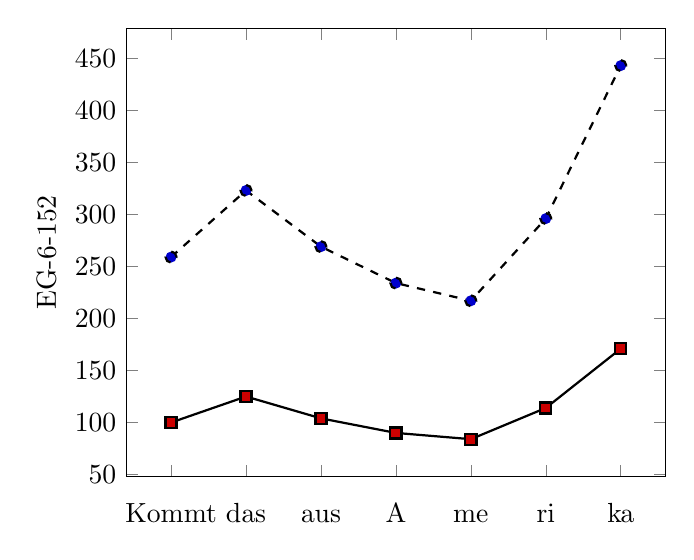
\begin{tikzpicture} 
\begin{axis}[symbolic x coords={Kommt,das,aus,A,me,ri,ka}  
	     ,ylabel=EG-6-152,
	     ,ytick={0,50,...,450} 	
	     ,xticklabel style= {anchor=south,yshift=-2em},
	    ] 
 \addplot+[black,dashed,thick] coordinates {(Kommt,259) (das,323) (aus,269) (A,234) (me,217) (ri,296) (ka,443)}; 
 \addplot+[black,solid,thick] coordinates {(Kommt,100) (das,125) (aus,104) (A,90) (me,84) (ri,114) (ka,171)}; 
\end{axis}

\end{tikzpicture}
\begin{tabular}{lrrrrrrr}
  \midrule
 Hertz     & 259 & 323 & 269 & 234 & 217 & 296 & 443 \\
 Percentage  & 100 & 25 & -17 & -13 & -7 & 36 & 50 \\ 
 Standard C. & 100 & 135 & 104 & 90 & 84 & 114 & 171\\
\end{tabular}~~~~~

\caption{Absolute and standard values of the melody \textit{Kommt das aus Amerika?} ‘Is this from America?’}
\label{graph:font:1}
\end{figure}

\begin{figure}
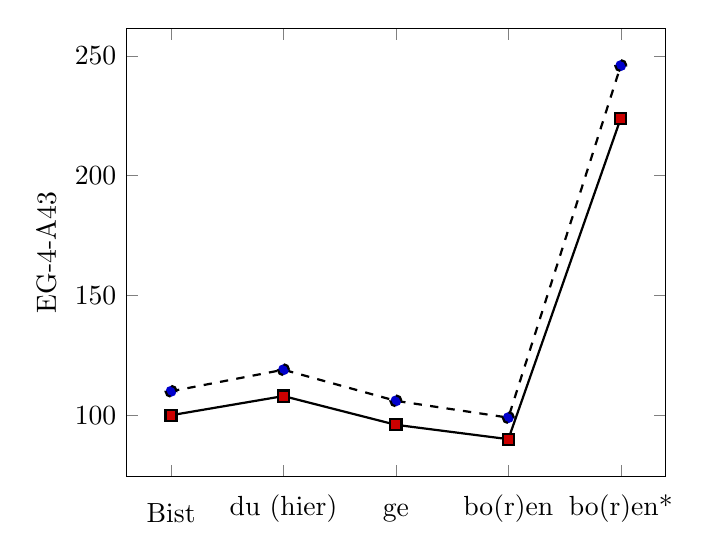
\begin{tikzpicture} 
\begin{axis}[symbolic x coords={Bist,du (hier),ge,bo(r)en,bo(r)en*}  
	     ,ylabel=EG-4-A43
	     ,ytick={0,50,...,450} 	
	     ,xticklabel style= {anchor=south,yshift=-2em},
]
 \addplot+[black,dashed,thick] coordinates{ (Bist,110) (du (hier),119) (ge,106) (bo(r)en,99) (bo(r)en*,246) }; 
 \addplot+[black,solid,thick] coordinates{ (Bist,100) (du (hier),108) (ge,96)  (bo(r)en,90) (bo(r)en*,224) }; 
\end{axis}
\end{tikzpicture}
\begin{tabular}{lR{1cm}R{1cm}R{.7cm}R{1.2cm}R{1.1cm}p{3mm}}
  \midrule
 Hertz       & 110 & 119 & 106 & 99 & 246  &\\
 Percentage  & 100 & 8 & -11 & -7 & 148 \\ 
 Standard C. & 100 & 108 & 96 & 90 & 224\\
\end{tabular}~~~~~

 
%\todo[inline]{Not sure about duplication of \textit{boren}. In case two different value are intended, here is a different graphic} 
% \begin{tikzpicture}
%\begin{axis}[symbolic x coords={Bist,{\color{white}a},du (hier),{\color{white}b},ge,{\color{white}c},bo(r)en,{\color{white}d}}]
%	\addplot+[blue,dashed] coordinates {
%		(Bist,110)
%		(du (hier),119)
%		(ge,106)
%		(bo(r)en,99)};
%	\addplot+[red,dotted] coordinates {
%		(Bist,110)
%		(du (hier),119)
%		(ge,106)
%		(bo(r)en,246)};
% 	\addplot+[smooth] coordinates { 
% 		(e,0)};
%\end{axis}
%\end{tikzpicture}
\caption{Absolute and standard values of the melody \textit{Bist du hier geboren?} ‘Were you born here?’  \label{graph:font:2}}
\end{figure}

With the application of this first phase of the method, or acoustic phase, we obtain the contour standardisation, which can now be compared and classified, regardless of the age, gender or any other characteristic of the speaker, as all the micromelodic variations have been removed and the values have been standardised. This process does not standardise the length of the different contours but isolates and replaces them with the number of tonal segments and their relative value, which is the only relevant data in a melodic analysis. The differences between two contours of different length should be understood from a melodic perspective, regardless of whether the melody contains a word or many words, whether it has a longer or shorter utterance, etc.

\subsection{Praat Script}
\label{sec:font:3.3}
This entire acoustic phase process that has just been discussed (sections 3.1 and 3.2), which includes the extraction and standardisation of the data and the creation of graphs, is done manually. In order to speed up the process, \citet{MateoRuiz.2010Scripts,MateoRuiz.2010protocolo} designed a script for Praat so that it could be done semi-au\-to\-mat\-ical\-ly.

To apply the script for Praat, first of all the corpus must be established, which can be in any language, dialect variety or register, taken from recordings of short and coded utterances. 

Once the script has been installed in Praat (see how to install in \citealt{MateoRuiz.2010Scripts}) the tonal segments for each audio file are established and labelled based on the creation of a TextGrid in Praat. This is a key point in the process as it requires precision and criteria in acoustic analysis. The work must be done using the expanded sonogram (selecting the ``Sel'' option) and in Pitch settings the option of speckles as drawing method must be enabled so that the limits of each tonal segment can be established with the greatest possible precision. At the same time the sound wave of the oscillogram must be considered, which reveals where the moments of maximum intensity are, corresponding to the tonal, in other words vowel, segments.

To create the labelling in TextGrid (see \figref{fig:font:4}), before the first segment of the utterance we must establish if it is a male (m) or female (f) voice. We can then begin to segment the first vowel of the utterance, which we transcribe with the first syllable. The aim is to search for the stable values of the vowel and mark the limits, which must be located after the first speckle of the vowel and before the last one, to ensure that the values are correct. To mark the limits of a syllable when it is a tonal inflection, either because the vowel has two or three values or because the syllable ends in a voiced consonant, we use the same criteria because the script will use the two, or where appropriate, three values.

Thus, in \figref{fig:font:4} we can see that the utterance is spoken by a woman (f) and that the first syllable is \textit{Bé} ‘Well’ in Catalan. We have marked the limits taking into account the stable values of the vowel 'e' and the point of intensity on the oscillogram, avoiding using values belonging to the previous voiced consonant, which is marginal. The second segment is the -\textit{i}- of \textit{cri}-. The voiceless occlusive -c- and the -r- prior to the vowel are not relevant values, as previously mentioned. Hence, the limits of the vowel are established respecting the same criteria. The same process is carried out for the other segments. The last vowel -\textit{ò} has a circumflex tonal inflection with three values. Also in this case we establish the limits at the beginning and the end of the vowel and the script will extract the three values. We can see the selection of the last two segments more clearly in \figref{fig:font:5}.

\begin{figure}
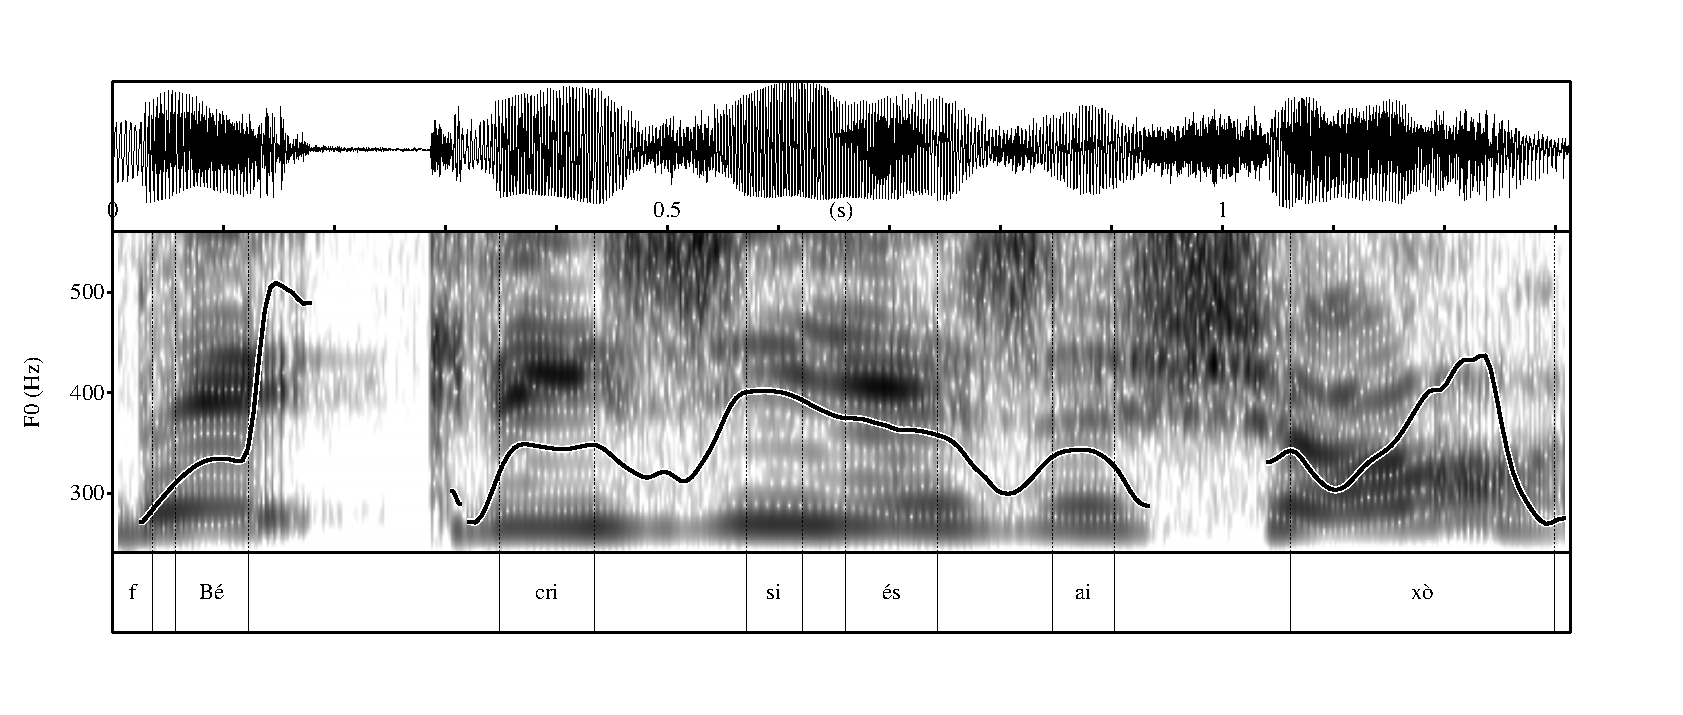
\includegraphics[width=\textwidth]{figures/FON-img6.eps}
\caption{\label{fig:font:4} Sonogram and TextGrid of the utterance in Catalan}  \textit{Bé, crisi és això}! 'Well, crisis is that!'
 
\end{figure}

\begin{figure}
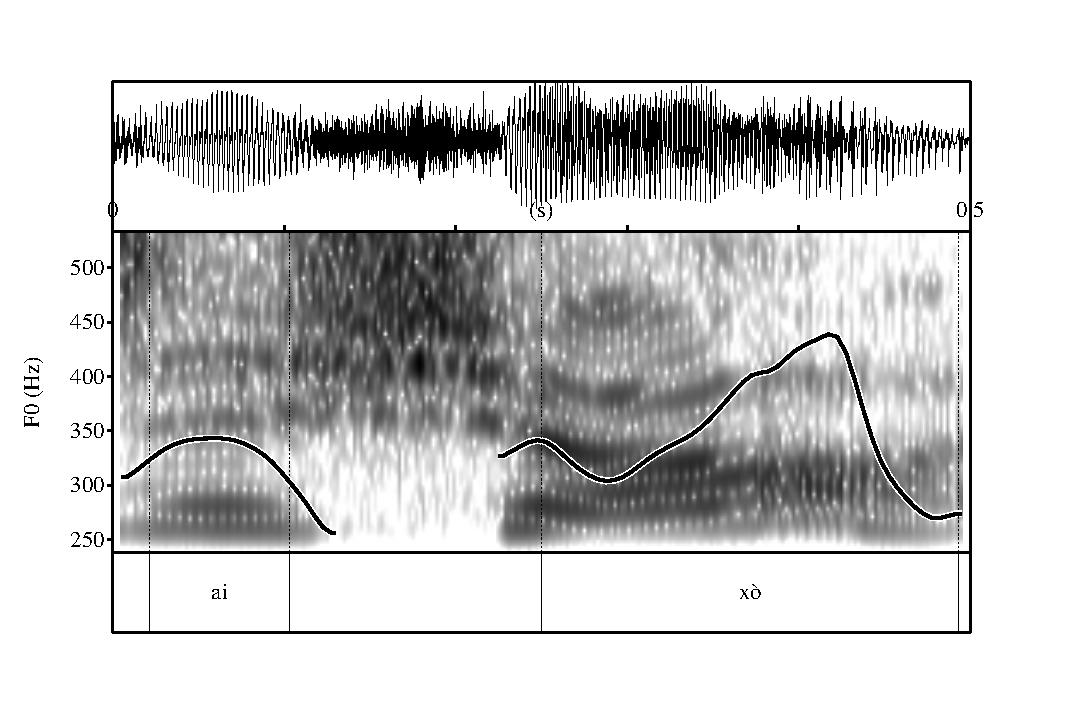
\includegraphics[width=\textwidth]{figures/FON-img7.eps}
\caption{\label{fig:font:5}  Last two tonal segments of the Sonogram and TextGrid of the utterance in Catalan  \textit{Bé, crisi és això!} 'Well, crisis is that!'
}
\end{figure}

The next step involves extracting the data, using the audio and the TextGrid of each one of the utterances. This is done by enabling the first of the scripts. This step must include a revision of warnings, such as values for segments that Praat cannot obtain or segments with three values that must be verified, among others, all of which will be flagged by the script. The subsequent modifications to the data, which may be necessary, must also be revised.

Once the correct data has been guaranteed, the standard curve of the utterance is created by enabling the second of the scripts and the graphs of the standard curve are generated using a macro in an Excel document provided by the script. Once the graphs have been created, comparisons can be made and the intonation models and patterns established\footnote{For more detailed information about the scripts, see \citet{MateoRuiz.2010protocolo}.}. See \graphref{graph:font:3}, in which a graph obtained by applying the script is shown.

\begin{figure}
\caption{Intonation curve of the Catalan utterance \textit{Bé, crisi és això!} `Well, crisis is that!'\label{graph:font:3}}
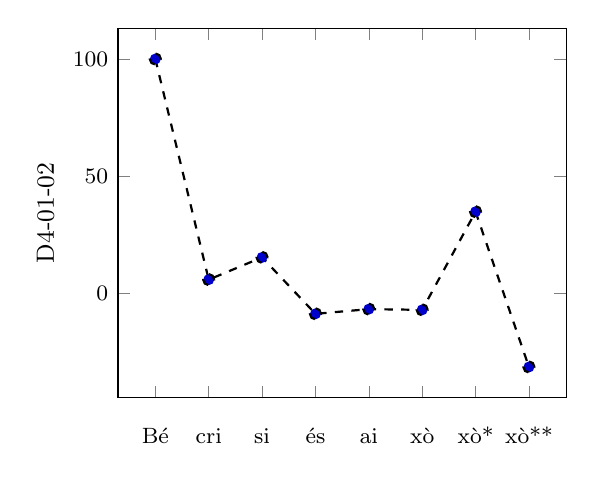
\begin{tikzpicture} 
\begin{axis}[symbolic x coords={Bé,cri,si,és,ai,xò,xò*,xò**}  
	     ,ylabel=D4-01-02,
	     ,ytick={0,50,...,450} 	
	     ,xticklabel style= {anchor=south,yshift=-2em}
	     ,small
	     ,width=.6\textwidth
	    ] 
%  \addplot+[black,dashed,thick] coordinates {(Bé,328) (cri,347) (si,400) (és,365) (ai,340) (xò,316) (xò*,426) (xò**,229)}; 
 \addplot+[black,dashed,thick] coordinates {(Bé,100) (cri,5.8) (si,15.3) (és,-8.8) (ai,-6.8) (xò,-7.1) (xò*,34.8) (xò**,-31.5)}; 
\end{axis}
\end{tikzpicture}
%\todo[inline]{code for the absolute graph is also provided if ever it is needed}

\end{figure}

In short, the Praat script is a reliable and simple tool that can be used to automate the data collection process for the analysis of intonation in any language and which saves researchers a considerable amount of time. However, before using the tool, acoustic analysis should be practised manually on a significant number of utterances in order to obtain criteria and to understand its characterisation.

After analysing all the contours and presenting them graphically, they must be classified into different groups according to the path of the final inflection (rising, falling, rising-falling, falling-rising, among others). For example, the representation of the two German contours (\graphref{graph:font:1} and \graphref{graph:font:2}) with a rising final inflection, characterises both as belonging to the same melodic class: contours with rising final inflection. In some cases, it must also take into account melodic features of the body and the first peak, such as the Spanish interrogative pattern, the rising body and final inflection pattern \citep{FontRotches.2013b}. Subsequently each group of contours must be organised according to the percentage of tonal movement in the final inflection, from greater to lesser, in order to apply the perception phase.

\section{Perception phase}
\subsection{Analysis validation} 
\label{sec:font:4.1}

In the perception phase, first of all the standard values of an intonation contour are validated in the voice synthesizer by ensuring that it has the same melody as the original, but with a different voice tessitura. We use the option ``To manipulate'' to open each contour in Praat’s programme in order to obtain this synthesised copy. After having opened a contour ready for manipulation (see \graphref{graph:font:5}), we erase all original data of the contour and replace it with our standardised data (see \graphref{graph:font:6})\footnote{In order to erase the original data, we must select it and erase clicking 'pitch' and 'remove pitch points' at the top of the screen. We can also replace it with our standardised data adding a dot where each vowel is located clicking 'pitch' and 'add pitch point at cursor'.}. We can check the validation of our results with a series of perception tests submitted to the listener’s judgement from an exact copy (thanks to voice synthesis) of the analysed sentences.

This validation of the melodies obtained during the acoustic phase of the analysis allows us to be completely sure that the analysis has been done correctly and that the obtained data are objective.

It also allows us to check that the validated melodies have been reduced to their most basic expression. Standardisation of the melodic curve provides us with the melody itself, regardless of the speaker’s tessitura and clean of any superfluous micromelodic variations. This method is very similar to \textit{close copy} by authors from the Dutch school \citep{Hart.1990}.

Following is an example, taken from research that defined the melodic patterns of interrogative intonation in Brazilian Portuguese \citep{CanteroSerena.2013}. The utterance \textit{Duzentos cinquenta os dois}? 'Two hundred and fifty for the two?', where the speaker is giving the price for two calves, revealed the following analysis (see \graphref{graph:font:4}). 

During the Manipulation process in Praat, the copy of the values is obtained (see \graphref{graph:font:5}) and the standardised values provided by the analysis are transferred to this copy (see \graphref{graph:font:6}).
We can now record the synthesis of the result and perceptively validate the melody.


\begin{figure}
\caption{Intonation curve of the Brazilian Portuguese utterance Duzentos cinquenta os dois?   'Two hundred and fifty for the two?'}
\label{graph:font:4}
\includegraphics[width=\textwidth]{figures/FON-img9.PNG}
\end{figure}


\begin{figure}
\includegraphics[width=\textwidth]{figures/FON-img10.PNG}
\caption{Copy of the original utterance.}
\label{graph:font:5}
\end{figure}


\begin{figure}
\includegraphics[width=\textwidth]{figures/FON-img11.PNG}
\caption{Standardised copy.}
\label{graph:font:6}
\end{figure}

\subsection{Identification of the melodic features} 
Once the melody of the intonation contours, obtained during the acoustic phase, has been validated, we can begin to identify its melodic features: the first peak, body or declination and the final inflection. Here it is important to distinguish between the different function that the contour's melodic features have, in the three levels of intonation analysis:

\protectedex{
\begin{itemize}
\item Prelinguistic intonation
\item Linguistic intonation
\item Paralinguistic intonation
\end{itemize}
}

\textit{Prelinguistic intonation} refers to the melodic features that allow the discourse to be structured and integrated in comprehensible units. The \textit{melodic profile} \citep{CanteroSerena.2011} of a language and of a dialect consists in this set of melodic features that characterise an ``accent'' (such as the dialect or foreign accent). The melodic profile of standard Peninsular Spanish, for example, coincides with the pattern of the intonation contour shown in \figref{fig:font:2}:


\begin{itemize}
\item a high first peak, whose centre is normally the first tonic vowel of the group (or the first post-tonic vowel);
\item a body or declination that falls evenly, with gradual inflections that systematically begin on a tonic vowel;
\item a final inflection that starts on the last tonic vowel of the group and can be falling (with values often greater than -15\%  ) or rising (with values that can reach more than +120\%). 
\end{itemize}

\textit{Linguistic intonation} refers to the level of intonation analysis that allows units that are different on a phonological level to be defined. For example, neutral intonation of interrogative, emphatic or suspended intonations, whose specific manifestations are the \textit{melodic patterns}, in other words, the melodies commonly used by native speakers of a language in their communicative interchanges and which can become models of production and perception.

\textit{Paralinguistic intonation} refers to the melodic features that provide a meaning related to the speaker's intentions or to the communicative context but which do not form linguistically coded units (although they can form semi-stable codes: see \citealt{CanteroSerena.2014}). We consider paralinguistic intonation to have a role in at least three well-defined areas:

\begin{itemize}
\item \textit{Emotional} intonation, including the expression of speaker's personal characteristics, his or her emotions and affection.
\item \textit{Focus} intonation, which centres on the actual melody of the utterance, to draw attention to it, focusing on it as a whole or on a part of it to underline its relevance in the discourse. A good example is the intonation of irony.
\item \textit{Politeness} intonation, which is focussed on the speaker and calls upon him or her to intensify or attenuate the effect of the message and, in general, to look for confrontation or cooperation.
\end{itemize}

In any event, there are very few melodic features of an intonation contour, therefore all of these functions are assumed by the same melodic features simultaneously. This is what we call \textit{melodic syncretism}. One same final inflection, which marks the end of the utterance and its \textit{linguistic} form (for example, an interrogation), can at the same time mark the speaker's dialect accent (\textit{prelinguistic}), express his or her concern (\textit{emotional}), focus on the question so that, in this context, it is clear that it is an ironic question (\textit{focus}) and reveal impoliteness to the listener (\textit{politeness}).

\subsection{Forming the hypotheses}
In order to establish the generalisations that allow us to understand how speech melodies work, based on the melodies obtained during the acoustic focus and validated perceptively, and once we have identified the melodic features we wish to test to determine their function, we will isolate them and identify the level of analysis to be referred to.

Only a perception test can guarantee which specific melodic feature is responsible for which prelinguistic, linguistic or paralinguistic, communication or discourse function.

For example, to determine the feature of the melody that is responsible for giving the utterance an interrogative value, we can isolate each one of the melodic values found in the analysis of corpus utterances that have been validated as ``melodies that confer an interrogative value''. If we confirm that the melodic feature common to all of them is a rising final inflection, we can determine that this feature, the rising final inflection, is the one we must test in the experiment. Therefore, based on the values that the melodic analysis provides for the questions analysed, we can formulate a hypothesis, such as: ``a rising final inflection conveys an interrogative value as of a specific percentage rise''. This hypothesis must be counter-verified in the perception test.

\subsection{Perception tests} 
Once the melodic feature to be tested has been identified, it is modified using Praat's synthesis routine (\textit{manipulation}). Using the previous example, we generate various identical utterances, in which only the value of the rise in the final inflection is modified.

We can modify an utterance in the corpus directly, as long as there are no grammatical, lexical, contextual parameters etc. that allow the sense or function of the melodic feature hypothesised as key for meeting this function to be identified. For example, we would not use phrases with an interrogative particle, however, we could choose a neutral utterance or create one ourselves by copying the standardised data and modifying only the feature to be tested (in this case, the final inflection).

Therefore, the modified melodic feature becomes the variable we wish to\linebreak counter-verify in the perception test. 

This test involves asking a significant group of listeners to react to the manipulated utterances. Various unmanipulated utterances, mixed with the manipulated ones (for example, with rises of 20\%, 30\%, 40\%, 50\%, etc. up to 120\%) and with other non-experimental utterances, in different perception sessions, with various groups of listeners. The results allow us to determine the percentage of rise that led listeners to the conclusion that the utterance is interrogative.

This procedure allowed the melodic patterns of Peninsular Spanish \citep{CanteroSerena.2007}  and Catalan \citep{FontRotches.2007} to be established for spontaneous speech. In \graphref{graph:font:7} we can see how the utterance used in the example in \sectref{sec:font:4.1} (in Figures \ref{graph:font:4}, \ref{graph:font:5} and \ref{graph:font:6}) is modified. In the original final inflection of the utterance there is a fall of 18.1\%. In the standardised copy (\graphref{graph:font:6}), we manipulate the last value (\textit{dois*}) and move from 118 Hz to 175 Hz, creating a rise of 21.5\% (equivalent to 158 in the standard curve). In this example, the final rise by 20\% did not allow us to identify the utterance as interrogative (as expected) but did as of a rise of 30\% (and up to 50\%). In Brazilian Portuguese, therefore, we can determine final rises with very slight interrogative values, which in Spanish or in Catalan are never understood as interrogatives: in Spanish, only as of 70\% and in Catalan as of 80\% \citep{CanteroSerena.2013}.

\begin{figure}
\includegraphics[width=\textwidth]{figures/FON-img12.PNG}
\caption{The last value is modified (in the circle) on the standardised copy of the contour and the final falling inflection (-18.1\%) is converted into a rising final inflection (+21.5\%).\label{graph:font:7}}
\end{figure}



\section{Discussion and concluding thoughts}
The theoretical assumptions of our method are not phonological, but exclusively phonetic, acoustic and perceptive: we determine the tonal segments that form the contour, we standardise their frequency values to express the melody and we validate them perceptively; we identify the melodic features that give the utterance different values (linguistic, pragmatic, discourse...) and we subject them to tests, to determine them; we work with tonal intervals expressed as percentages (equivalent to semitones, but more easily and more intuitively handled), etc.

Therefore, it is an independent method, which is at the same time compatible with any phonological focus (structural, notional, autosegmental, etc.), particularly with methods of phonological labelling as ToBI. The melodies resulting from the analysis have the advantage of allowing any speaker to be compared, of handling large quantities of data and of establishing reliable statistics and precise dispersion margins thanks to the exact quantification of the intervals.

This makes it a solid method: it allows the analysis of spontaneous speech, it requires no preliminary alignments and works well with all types of corpus. It is also objective: the perception test ensures that all of the standardised values and resulting melodies are reliable.

Compared to other intonation analysis models, MAS allows:

\begin{itemize}
\item Study of intonation from exclusively phonetic levels of analysis, which do not require the use of other levels of linguistic or grammatical analysis, nor do they depend on them.
\item Work with a formal analysis method, based on the acoustic and perceptive analysis of speech. This analysis provides a description of the intonation from a strictly phonetic viewpoint, which is very detailed, regardless of its phonological interpretation.
\item Characterise not only standard melodies of a language or dialect (whose phonetic generalisation is possible in the perceptive, experimental phase of the method), but also the individual variants of a single speaker and even the characteristics of pathological speech.
\item Work with spontaneous speech: although any type of corpus can be used in the analysis, the solidity of the method allows large volumes of data and a wide range of anonymous speakers to be handled.
\item Use the open phonetic analysis method, which allows any type of notation, analysis or subsequent transcription: pragmatic, grammatical, lexical, as well as any type of phonological labelling. For example, the Autosegmental-Metrical model (AM), which has a labelling convention known as \textit{Tones and Break Indices} (ToBI), is a phonological labelling method for intonation, not a phonetic analysis method. In this sense, it is completely compatible with the MAS method. See two examples in  \graphref{graph:font:8} and \graphref{graph:font:9} which demonstrate the compatibility.
\end{itemize}

\begin{figure}{}
\includegraphics[width=\textwidth]{figures/FON-img13.PNG}
\caption{Contour phonetically analysed with the MAS method and labelled with the SP-ToBI system.}
\label{graph:font:8}
\end{figure}

According to MAS method, the melodic contour of Spanish \textit{¿Tiene usted hijos?} (see \graphref{graph:font:8}) is characterized by a flat body, without anacrusis and first peak and a rising-falling final inflection. This flat body is phonologically transcribed as L* in AM model because it is phonetically realized as a low plateau at the minimum of the speaker’s range. And the melody of the final inflection has a tonal rise of 28,3\% from the first value of the nucleus, \textit{hi-}, to the second, hi-*  and a tonal fall of 18,9\% from the syllable \textit{hi-*} to \textit{-jos,} which are produced with an L+H* nuclear accent followed by a boundary tone, L\%. As we have seen in graph 8, we can label the melodic contour according to Sp-ToBI based on \citet{Beckman.2002} and later revised by \citet{FacePrieto.2007} and \citet{EstebasVilaplanaPrieto.2008} and is totally compatible.

\begin{figure}
\includegraphics[width=\textwidth]{figures/FON-img14.PNG}
\caption{Contour phonetically analysed with the MAS method and labelled with the SP-ToBI system.}
\label{graph:font:9}
\end{figure}

We can see another example in \graphref{graph:font:9}. The melodic contour of the question \textit{¿Usted es de Gran Canaria?} starts with an anacrusis with a tonal rise of 68\% until the first peak, \textit{es}, which is displaced in the unstressed segment after the first stressed segment of the contour, \textit{-ted}. After that, the melodic line is going down abruptly until the nucleus, \textit{-na-} and ends with a falling final inflection of 14,6\%. These phonetic features can be complemented with a phonological description in the AM model: an L+ <H* prenuclear pitch accent, which involves a rise with a displaced F0 peak, an H+L* nuclear accent, realized as a F0 fall within the accented syllable, and an L\% boundary tone. 

In short, MAS is not an alternative method for the analysis of intonation but is simply ``the acoustic analysis of the melody'', the phonetic analysis method for intonation which can be complemented with a phonological description.

In fact, carrying out a detailed acoustic analysis of the melodic features of speech is a laborious task and this is undoubtedly the main disadvantage of the method. For this reason we suggest simplifying the analysis process using the Praat script described in \sectref{sec:font:3.3}, which we continue to optimise to facilitate the task. Many authors have preferred to limit themselves to an intuitive approach to the melodic curve, expressing only the pitch levels that may have a phonological relevance, the assumed stresses and the limits of the utterance. This is a reasonable method when there is no need for a detailed analysis of the melodies but simply their phonological expression. However, just as the acoustic analysis of the segments cannot be replaced by their simple transcription, on occasion there is a need for a detailed melodic analysis. For example, to characterise the intonation of foreign speakers of a language, to describe dialectal intonations, to distinguish personal characteristics of a speaker, or to specify the melodic features that have pragmatic or discourse functions, etc. In all of these cases, where there is a need to go beyond the previously deduced phonological characterisation, a detailed melodic analysis must be made. Also, clearly, when the researcher wishes to establish linguistic generalisations based on the mass analysis of new acoustic data.

Since it was proposed \citep{CanteroSerena.1999} and to date, the method has been used with success in different studies, by our research team\footnote{See a compendium of the first ten years of work in \citet{VariousAuthors.2009} and a more recent revision in \textit{Phonic} magazine, vol. 9-10 (2013-2014). \url{http://revistes.ub.edu/index.php/phonica/index}} and by different international research groups (particularly South American).

At our research centre, the University of Barcelona's Applied Phonetics Laboratory\footnote{\url{http://www.ub.edu/lfa/}}, we have created a wide corpus of spontaneous speech for Peninsular Spanish and Catalan, among other languages (see \sectref{sec:font:2.3}).

Overall, research on the following areas has been carried out:

\textit{Prelinguistic intonation}: dialect accents of Peninsular Spanish \citep{BallesterosPanizo.2011,MateoRuiz.2014} and Catalan \citep{FontRotches.2014b,PonsLlabres.2014}; as well as for various interlanguages (foreign accents): the intonation of Spanish spoken by English \citep{MunozDuarte.2014}, Swedish \citep{Martorell.2010}, Hungarian \citep{BaditznePalvoelgyi2012}, Italian \citep{Devis.2011a}, Brazilian \citep{FonsecadeOliveira.2013} and Chinese \citep{CortesMoreno.2004,Liu2005} speakers; and the study of speech demarcation units for Spanish \citep{CabedoNebot.2013,MartinezHernandez.2015, MasManchon.2008}.

\textit{Linguistic intonation}: melodic patterns and dispersion margins for Peninsular Spanish \citep{CanteroSerena.2007}, Cuban Spanish \citep{GarciaRiveron.2010}, Catalan \citep{FontRotches.2007}, Brazilian Portuguese \citep{Araujo.2014,CanteroSerena.2013,Silva.2009,Mendes.2013}, German \citep{TorregrosaAzor.2011,TorregrosaAzor.2015,TorregrosaAzor.2016} and Chinese \citep{Kao.2011}.

\textit{Paralinguistic intonation}: focusing on politeness and impoliteness for Spanish \citep{DevisHerraiz.2011phonica} and Catalan \citep{DevisHerraiz.CanteroSerena.2014}; mechanisms of focus in Peninsular Spanish \citep{CanteroSerenaETAL.2005}, South American Spanish \citep{Pereira.2014,RuizMella.2011}, Catalan \citep{FontRotches.2011,FontRotches.2014} and of professional speakers \citep{FontRotchesMachucaAyuso.2010,FontRotchesMachucaAyuso.2010,FontRotchesPaloma.2013,Torrent.2012,Torrent.2015}; and an initial approach to emotional intonation \citep{CanteroSerena.2014}.

Much of this research is still on-going. Currently, work is being made on melodic patterns for Portuguese, German and English, as well as different studies on dialects of Catalan and American Spanish. We have also begun working on the educational applications of our intonation research, particularly on paralinguistic intonation: \citet{DevisHerraiz.2015,DevisHerraiz.Bartoli.2015}.

Among the urgent research tasks we propose is the implementation of the script for Praat, in a new version that goes beyond melodic analysis and allows the standardisation of the intensity (dynamic analysis) and of the duration, which would allow a complete \textit{prosodic analysis} of speech.

In effect, our method only allows the analysis of melodies. However, as we look further into the analysis of spontaneous speech and the prelinguistic and paralinguistic levels of intonation we find differences that go beyond the strictly melodic, related to the dynamics and the relationships of duration between the melodic units, which doubtless play a very important role in speech. 

Therefore, the next step we will take in the analysis of intonation will be the Prosodic Analysis of Speech.


{\sloppy
\printbibliography[heading=subbibliography,notkeyword=this]
}

\end{document}
